\title{\textbf{The Automatic Toilet Freshener \\ \large \emph{A technical odyssey}}}

\author{Bastiaan Weijers \\ 3256669 \and Colin Smits \\ 4075390}
\date{}
\documentclass[a4paper, 12pt]{article}
\renewcommand{\familydefault}{\sfdefault}
\usepackage{enumitem}
\usepackage{graphicx}
\usepackage{pdflscape}
\usepackage{hyperref}

\begin{document}
\maketitle

\section{Introduction}
How to write a piece of code that controls something that is used daily, and how to make this usable in real life? That was the question we asked ourselves at the beginning of this project. What is it like to create your own piece of hardware, and how to connect all the sensors and actuators in the right way? We explored all these things in the project as well. But above all, this paper will describe the flow we had working through the project of controlling an automatic toilet freshener using an Arduino soldered and put together ourselves, covering all our thoughts and opinions on the subject of using the sensors the right way. In the first part, we will cover the technical details, such as the states used, the possibilities we thought we had to define these states using the sensors, and the final decisions upon the use of the sensors. After that, we'll discuss the development of the circuit, along with the difficulties involved. Finally, we'll describe how our creation works under normal operation, and reflect on the final product and the way we got to this. 

\section{Technical Overview}

%include state diagrams, circuit

\subsection{States}
\label{sub:state}
To start off with the technical details, we need to define states in which are system can be operating. These states must be defined according to the usage of a toilet. So, just after trying out all the circuits with the sensors, we started thinking about distinctive features of a toilet use. 

First of all, you would have to open a door in order to get into the toilet. After that, you would maybe turn on the light in order to see where you are heading, making sure you do not miss the seat and fall down and/or need to clean the floor afterwards. These are the first two point that would suggest the usage of a toilet.

Secondly, you might need to open the lid in order to be able to sit down, or, in the case of a male user, you might need to put the seat up in order to have an increased target area. These are indications of the type of use, while a standing person would not attempt a "Number 2" usage (if you still have a normal functioning brain). Some people might close the lid again after usage, which would indicate they are done using the toilet, setting a time reference for our future system.

After using the toilet, you should be flushing and leaving the area. Therefore, you would open the door (if you did not close it \ldots) and turn off the light (if you actually turned it on \ldots). These are indications of the end of an usage, which would require the freshener to do its job and clear the area of "bad smells".

\subsection{States of the Sensory}
In \S\hyperref[sub:state]{\ref{sub:state}} we defined the general use case of a toilet system. Now we need to turn these transitions into factors which we can measure using our sensors. 

Starting off with the entrance, we can see that we could place a \textbf{magnetic sensor} in the door opening to measure the state the door is located in. Furthermore, we can measure the amount of light in a room using our \textbf{Light Dependent Resistor} (LDR). A sudden increase of light \emph{might} indicate a person entering the room. You are even more certain when the door is being opened and closed almost simultaneously, but still there is no guarantee. As we will see later on, you can never be sure what a person is doing inside the toilet (\ldots).

As we stated as well, a person might need to open the lid. If we were to place the \textbf{magnetic sensor} on the lid, we might be able to see whether the toilet is being used even more carefully. In order to be able to decide if a person is sitting or standing, we can use the \textbf{distance sensor}. In general, a standing person is further away from the wall behind the toilet then a sitting person.

Using these possible positions we head for the farewell of the toilet for now. We can measure whether a person is gone away from the toilet by using the \textbf{distance sensor} again. After finishing someone might close the lid (\textbf{magnetic sensor}) and walk through the door (\textbf{magnetic sensor} possibly) and turning off the light (\textbf{LDR}). 

\subsection{Decisions, decisions}

We have set out all the possible uses for our sensors. In the end, we decided to do the following placements:
\begin{description}
\item[Distance Sensor] We place the \textit{distance sensor} on the wall behind the toilet to measure the distance between the wall and a person.
\item[Magnetic Sensor] We place the magnetic sensor on the flush button. By doing this, we can verify once more whether the toilet has been used, and when the user is starting to leave the toilet.
\item[LDR] We locate the \textit{LDR} close to the light source in the toilet to measure the on/off transition of the light.
\end{description}

\noindent After setting the locations, we are able to define our state diagram. However, we still need to make sure that the other components are used as well:
\begin{description}
\item[Temperature sensor] Located somewhere in the toilet just to measure the temperature. Is not used in deciding the states.
\item[Push Buttons] Two of the push buttons will be used for menu control, setting the delay of the spray as well as a reset for the spray counter. The other push button will be the manual override for a spray.
\item[LEDs and LCD Screen] All of these will be used as indicators for states and feedback towards the user.
\end{description}

Our final \hyperref[fig:stateDia]{state diagram} can be seen at the end of the paper.

\section{Development}
\subsection{First circuits}
In order to create a system that is able to do such a difficult task, we had to be able to create the circuits. As we were progressing through all the sensors, one of us hooked up his temperature sensor for testing purposes. It was then that we noticed a smell. The LCD display was not able to tell what it was, because it had no power. We pulled the USB cord from the computer immediately, as the smell was intensifying. After touching the temperature sensor, it became clear that this was the source: it was too hot too handle. This was the first piece which was harmed (but not destroyed), and in the full process of developing, some other pieces would fall victim to bad wiring.

\subsection{The final circuit}
After a week of intense coding and caffeine intake, along with some shocking progress on the circuit, we had created our final circuit without the refresher hooked up yet. We found that our code was fairly able to define our states, so we decided to give it a try. It was then we victimized the second part of our kit: after an hour of trying to get the refresher to work on pin 13, we found that the circuit didn't work, as the led was on, but there was no current going through the refresher. So we decided to replace the parts one by one, only to find out that the MOSFET was not working any more. Luckily, we had been equipped with two sets, so we replaced the MOSFET. We then had our circuit fully working, as can be seen in  \hyperref[fig:circuit]{Fig. 1}. A final setback came in the last instalment, when we found out that one of our motion sensors had broken down as well. This, too, was fixed by a replacement.

To make sure we were able to incorporate all the parts, we have decided to put the push buttons on the analogue inputs as it was fairly easy to code the buttons from there as well. Along with that, we had to put two of the LEDs on the analogue inputs due to lack op space. The decision was made as well to hook the refresher onto pin 13, so that the LED on the Arduino itself would be activated in line with the refresher, so it's easy to see when the refresher is active.

\begin{figure} \label{fig:circuit}
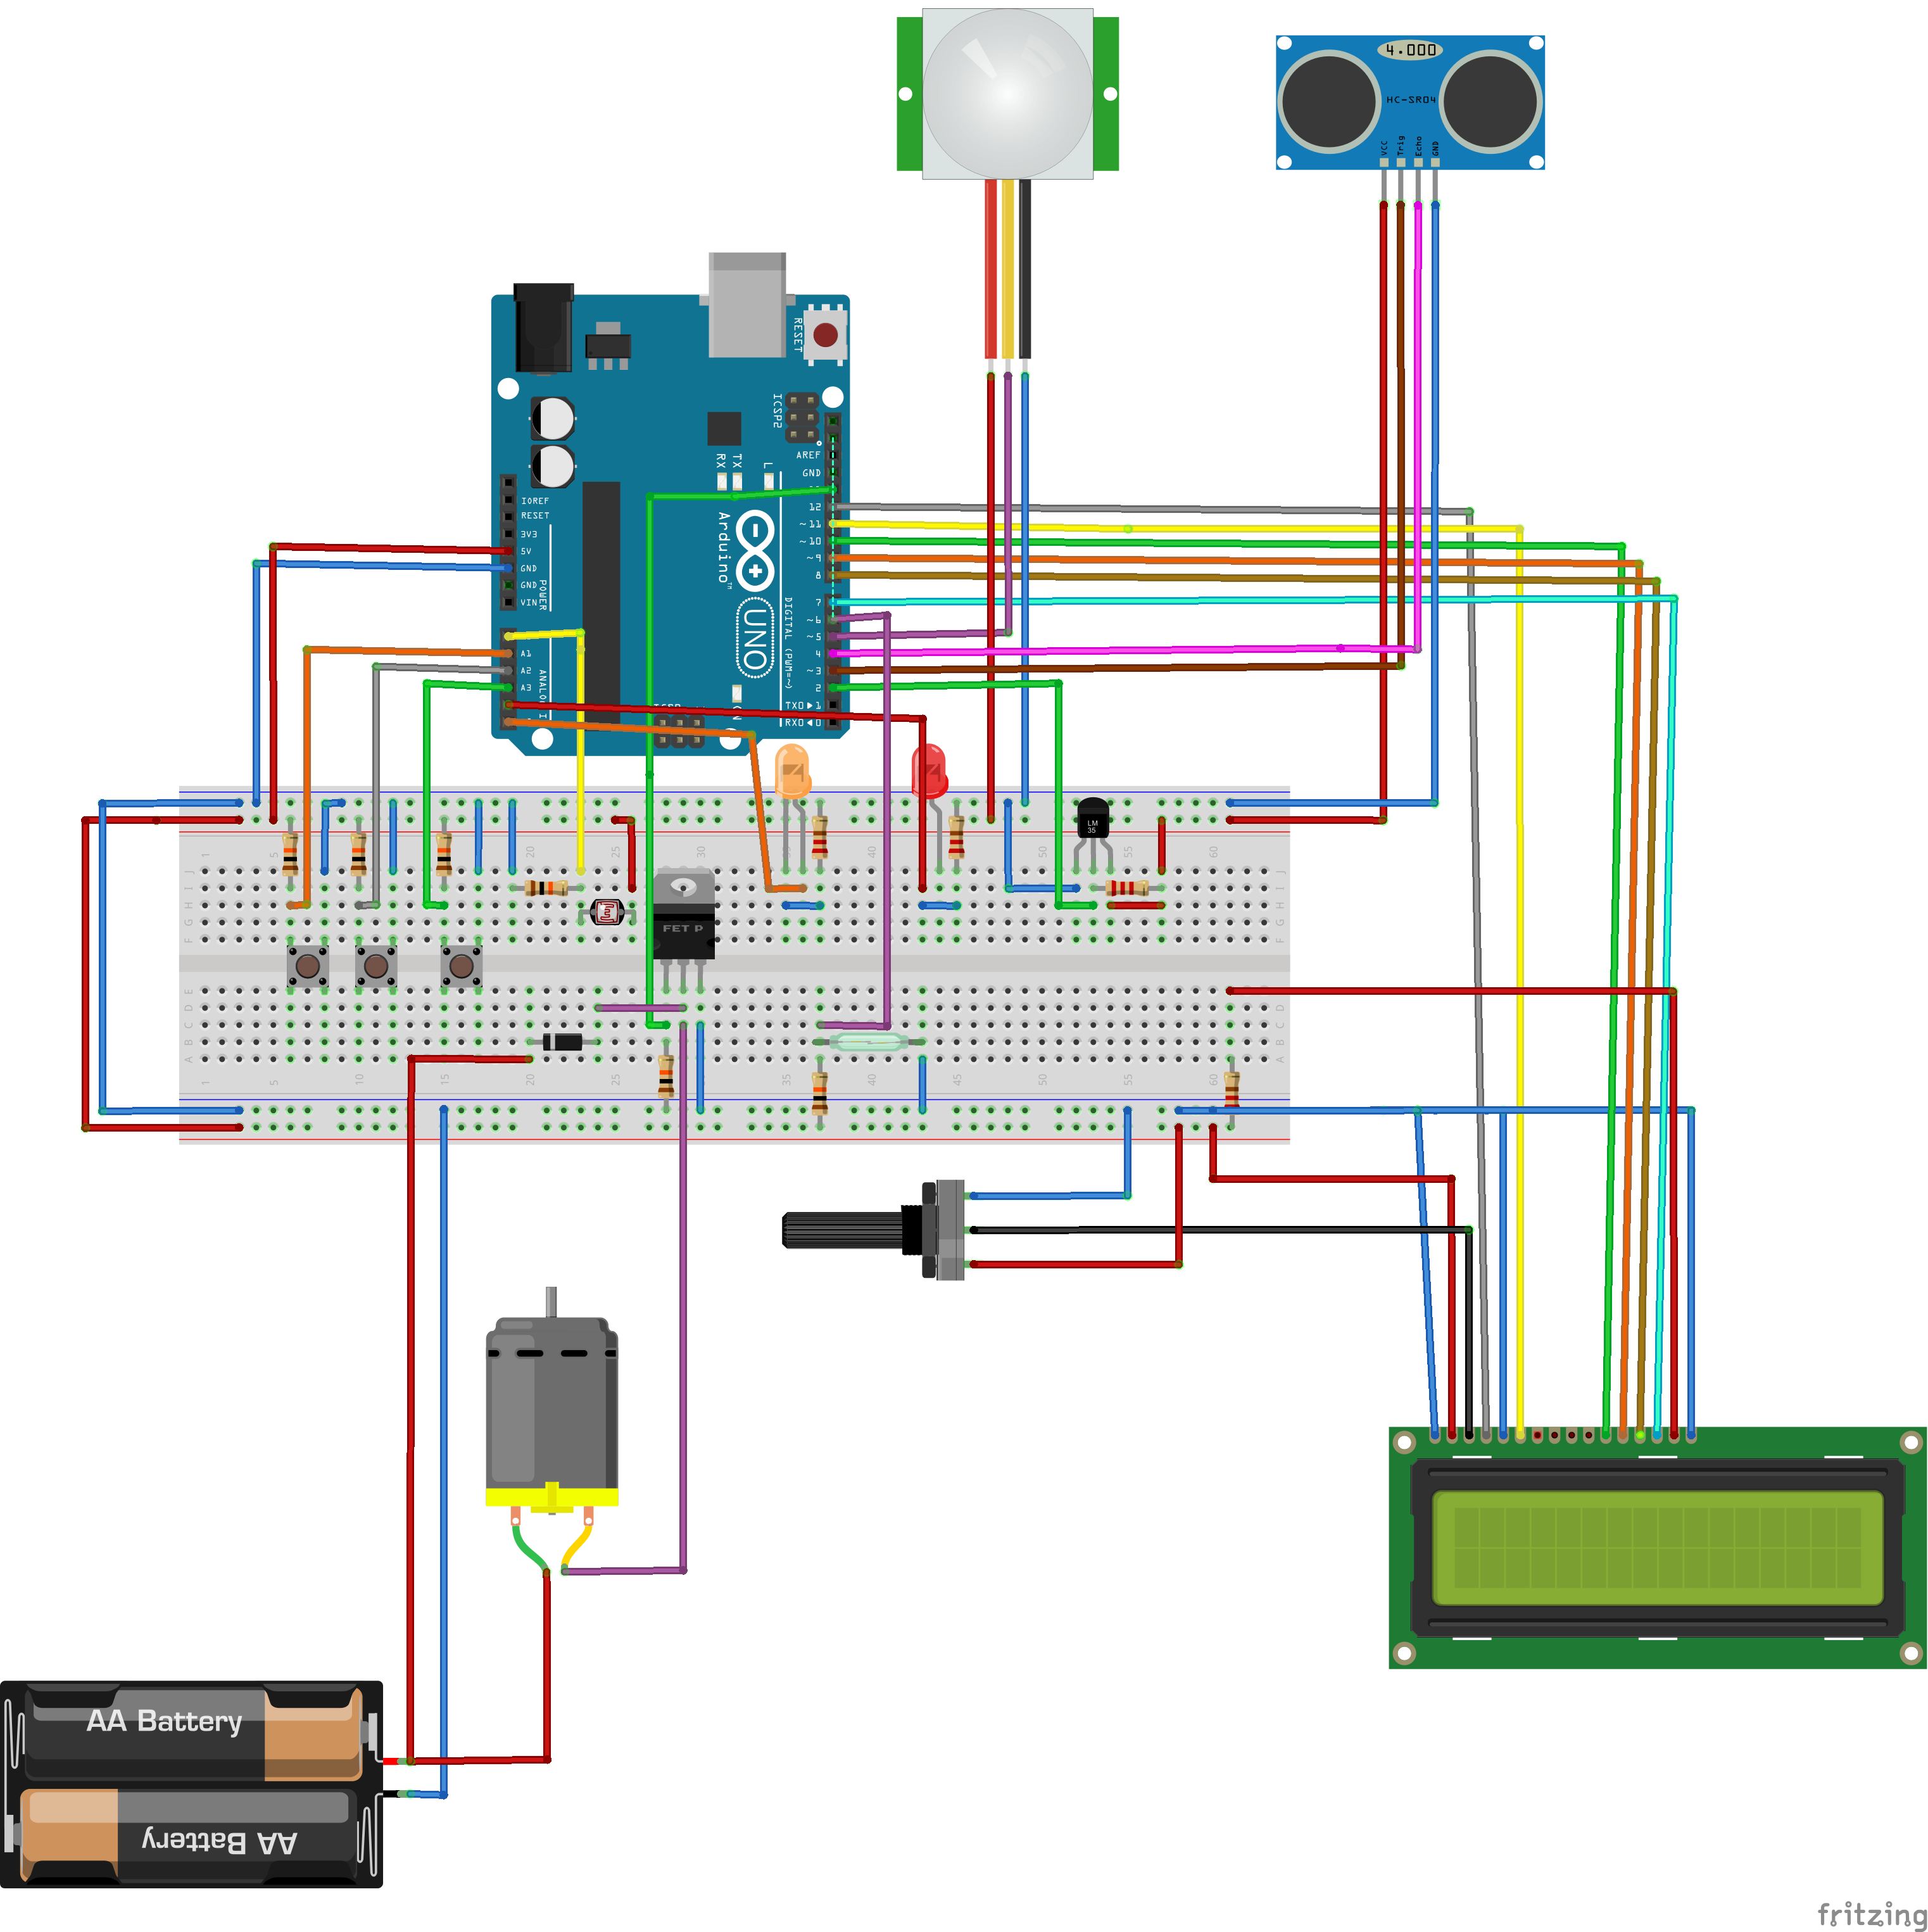
\includegraphics[scale=0.4]{schakeling_bb.png}

\caption{The breadboard circuit of our system}
\end{figure} 

\section{Usage}
Our refresher actually works using the distance and motion sensor along with the magnetic sensor. We decided that we could keep track of time during usage by measuring the time someone is within a certain distance from the wall. For example, we would be 30 cm away from the wall when sitting, and 70 cm when standing. We used these to distinguish between a number 1 and number 2 for a male use. Along with that, we thought we could use a time indication for stating whether someone had been doing a number 1 or number 2. We set the time for a number 1 to a minimum of 20 seconds, and a number 2 to a minimum of 45 seconds. Along with that, we measure the time the user is sitting, and when this does not meet the minimum for the number 2, a number 1 is called.

In between the transitions of sitting and standing, we decided we had to use a decision "delay". For example, when I am sitting on the toilet, and for some reason I have to reach out, I might be out of sitting range for a second. This should not be triggering a transition of sitting to standing. Therefore, we have a frame in which the decision is made: if state A turns to state B, we wait to see if after 2 seconds still a state B is in place. Then is the time we switch.

\subsection{Indications}
During normal operation, the LCD screen will display the current ambient temperature, which is refreshed every 2 seconds. Besides, it shows the amount of sprays that should be left within the refresher. 

Almost every state is indicated using the LEDs:
\begin{description}
\item[Red only -- continuous] indicates movement is being registered.
\item[Red / Yellow -- continuous] indicates someone is using the toilet.
\item[Red/Yellow -- blinking rapidly] indicates a standing person (number 1).
\item[Red/Yellow -- blinking slowly] indicates a sitting person (number 1 / number 2).
\item[Yellow -- continuous] indicates end of usage (ready to spray).
\item[Red LED on Arduino along with Yellow] indicates power is running through the refresher. This LED is turned on 15 seconds before the spray is given (due to the delay within the refresher).  
\end{description}

When a spray is to be given, a countdown will be displayed on the LCD screen, telling the user when the spray will be delivered (so he has time to run away).

\subsection{Menu and  manual spray}
Our system is able to be controlled by the user whilst operating. When the user hits the menu button, the system will show a menu screen. When the user hits the menu button again, the system will scroll through the different options available:

\begin{description}
\item[Resetting the spray count:] The user can reset the spray count by selecting the right menu, and toggling the presented option (True / False] by hitting the select button. After a change of selection, a countdown of 5 seconds is triggered, in which the user can still switch. after the 5 seconds have expired, the system will return to normal operation.
\item[Setting the spray delay:] The user can also set the delay (in seconds) after which a spray is delivered. Due to the technical shortcomings of our refresher, the delay can only be set in the interval $[15, 63]$ seconds. The timer is increased by 1 each time the select button is hit.
\end{description}

Along with the on-board menu, we have a dedicated push button which triggers a spray manually. After the user hits this button, the system will stop its current operations, and get into the spraying state. The spray is delivered at exactly the delay defined by the user in the menu.

\section{Reflection}

As to conclude, we look back to how well the project went. We headed off for a strong start, as we had all the components working after only 3 days, so we started building in the first week already. At first, we thought it would work out well at once, and there would be not much of a hassle finishing the project. As time progressed, we actually found that coding for an Arduino involves more skill than just thinking in methods, as you are building upon lots of timers. Moreover, the components of the sensor kit started to work against us, leading to two casualties, as we have stated previously.

Due to the underestimation of the work, we were not able to full incorporate all the sensors into the coded state machine. However, we managed to create a working prototype with the materials we had (as you can see in the short film). All in all, we think we did the best we can and we have encountered what it means to work with hardware instead of only writing code.

%state diagram in landscape mode

\newpage
\begin{landscape}
\begin{figure}[h!]
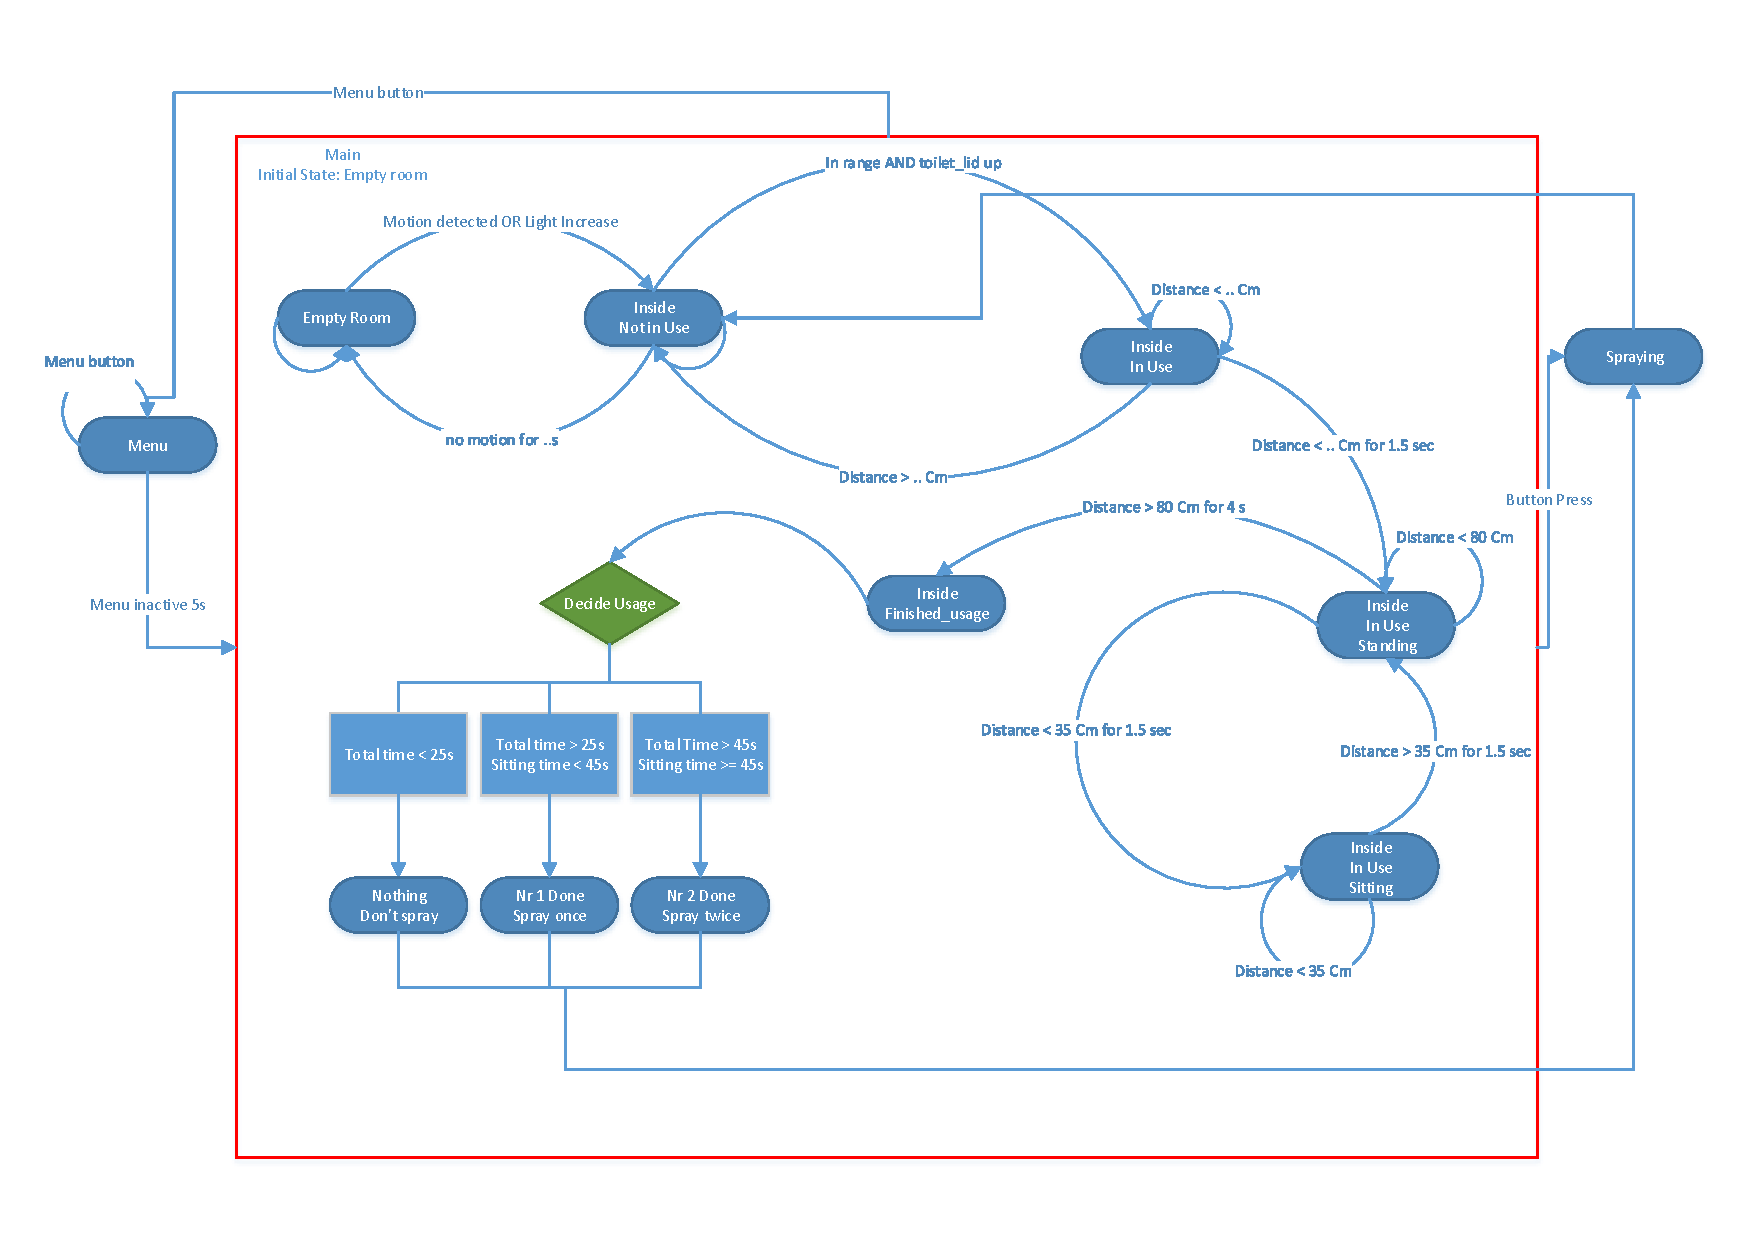
\includegraphics[scale=0.75]{State_Diagram.pdf}
\label{fig:stateDia}
\caption{State Diagram of our system}
\end{figure}
\end{landscape}



\end{document}
